\documentclass{article}
\usepackage[utf8]{inputenc}
\usepackage[T1]{fontenc}
\usepackage{lipsum}
\usepackage{graphicx}
\usepackage{amsmath}
\usepackage[margin=1in]{geometry}
\usepackage{titlesec}
\usepackage{enumitem}
\usepackage{geometry}
\usepackage{tabularx}
\usepackage{caption}
\usepackage{fixltx2e}
\usepackage{booktabs}
\usepackage{float}  % Aggiunto pacchetto float

\titleformat{\section}
{\LARGE\bfseries}{\thesection}{1em}{}

\titleformat{\subsection}
{\Large\bfseries}{\thesection}{1em}{}

\begin{document}

\pagestyle{empty}

\section*{ESQL}
\large
Nella qui presente documentazione si riportano l'insieme delle specifiche necessarie per comprendere al meglio la direzione seguita dallo sviluppo del progetto \textbf{ESQL}. Si susseguono sezioni relative alla modellazione, espandendosi da tematiche inerenti alla progettazione di entità-relazioni fino all'adozione dei modelli concettuali, logici e fisici.

\subsection*{Modello E-R}
\begin{figure}[H]
    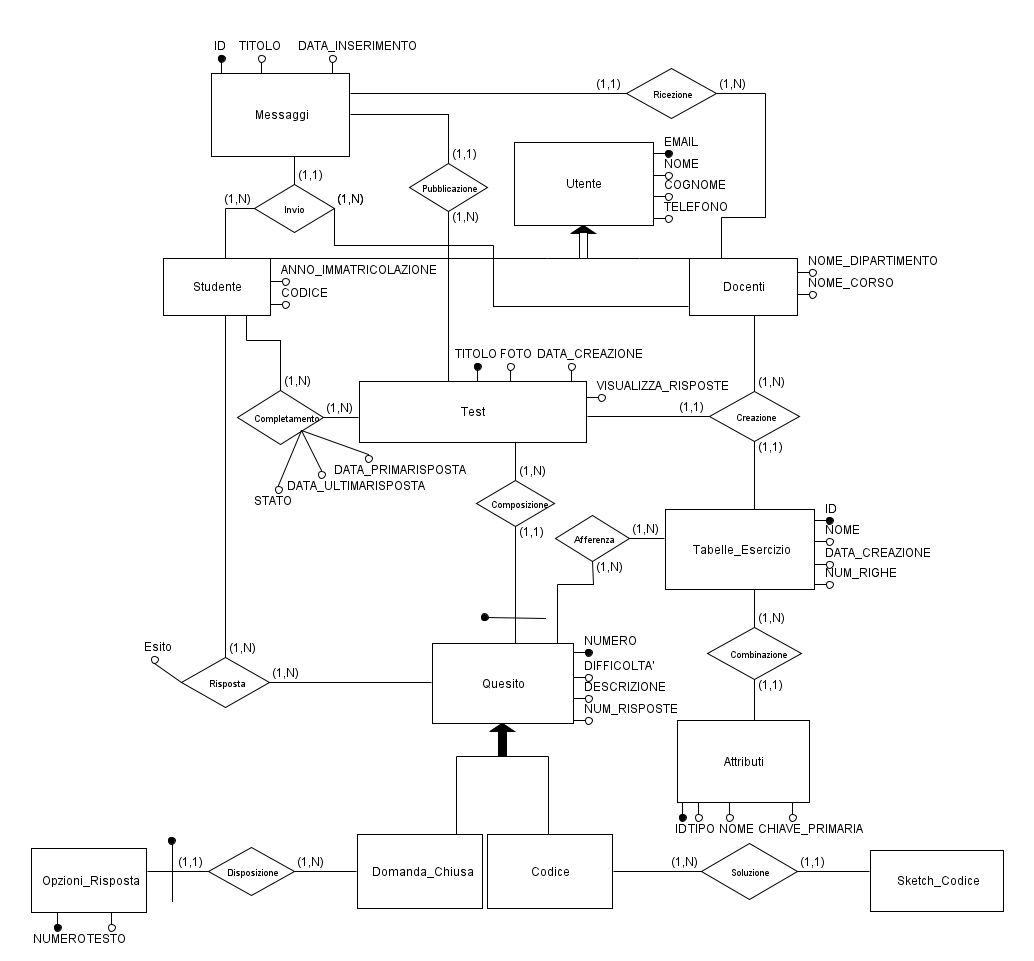
\includegraphics[width=1.1\textwidth]{foto1.png}
    \caption{Modello E-R precedente alla raffinazione.}
\end{figure}

\subsection*{Dizionario delle entità}
\begin{table}[H]
    \centering
    \begin{tabularx}{\textwidth}{|X|p{5cm}|X|X|}
        \hline
        Entità & Descrizione & Attributi & Identificatore \\
        \hline
        Utente & Utente rappresenta coloro che adoperino il software realizzato & Email, Nome, Cognome, Telefono & Email \\        
        \hline
        Docenti & Sottotipo dell'entità padre Utente, da cui si delineano specifiche attività che possano essere conseguite & Nome\_Dipartimento, Nome\_Corso & Email \\
        \hline
        Studente & Sottotipo dell'entità padre Utente, il quale si contraddistingue per certe azioni che possano esercitare & Anno\_Immatricolazione, Codice & Email \\
        \hline
        Tabelle\_Esercizio & Definisce i meta-data necessari per la creazione vera e propria di relazioni & ID, Nome, Data\_Creazione, Num\_Righe & ID \\
        \hline
        Attributi & Definisce i meta-dati necessari per la concretizzazione di tabelle inerenti alla creazione di esercizi da sottoporre successivamente agli Studenti & ID, Tipo Nome, Chiave\_Primaria & ID \\
        \hline
        Test & Test entità necessaria per sottoporre gli Studenti alla risoluzione di possibili quesiti & Titolo, Foto, Data\_Creazione, Visualizza\_Risposte & Titolo \\
        \hline
        Quesito & Entità fondamentale per la creazione delle domande da sottoporre agli Studenti, raggruppati in specifici test & Numero, Difficoltà, Descrizione, Num\_Risposte & Numero \\
        \hline
        Risposta & Entità idealizzata per salvaguardare e verificare le risposte formulate dagli Studenti in merito a quesiti specifici & ID, Esito & ID \\
        \hline
        Domanda\_Chiusa & Tipologia di Quesito, la quale rappresenta una domanda a scelta multipla & . & Numero \\
        \hline
        Sketch\_Codice & Tipologia di Quesito, necessita la formulazione di codice SQL che restituisca righe e colonne attese & . & Numero \\
        \hline
        Messaggi & Relazione ideata per mantenere al suo interno comunicazioni inviate e ricevute da Studenti e Docenti mediante l'impiego di applicativi & ID, Titolo, Data\_Inserimento & ID \\
        \hline
    \end{tabularx}
    \caption{Descrizioni delle entità della prima stesura del modello E-R}
\end{table}

\subsection*{Dizionario delle relazioni}
\begin{table}[H]
    \centering
    \begin{tabularx}{\textwidth}{|X|p{5cm}|X|X|}
        \hline
        Relazione & Descrizione & Componenti & Attributi \\
        \hline
        Creazione & Adottata per la concretizzazione da parte dei Docenti delle tabelle e test di esercizio & Docenti, Tabelle\_Esercizio, Test & . \\
        \hline
        Realizzazione & Gli Studenti formulano possibili risposte rispetto ai quesiti posti dal test & Studente, Risposta & . \\
        \hline
        Completamento & Relazione ideata per tenere traccia degli Studenti che partecipino allo svolgimento dei test sottoposti dai Docenti & Studente, Test & Stato, Data\_UltimaRisposta, Data\_PrimaRisposta \\
        \hline
        Invio & Associazione necessaria per il consecutivo smistamento di messaggi tra Studenti e Docenti & Studente, Docenti, Messaggi & . \\
        \hline 
        Pubblicazione & Tramite per associare possibili messaggi rispetto ai quesiti posti all'interno di uno specifico test & Messaggi, Test & . \\
        \hline
        Ricezione & Relazione attuata per stabilire quale sia il docente ricevitore di comunicazioni da parte dei propri Studenti & Messaggi, Docenti & . \\
        \hline
        Svolgimento & Stabilita per formalizzare quali risposte siano collegate alle domande poste in certi insiemi di quesiti & Risposta, Quesito & . \\ 
        \hline
        Composizione & Un insieme di quesiti specifica una determinata Test, imponendo in questo modo un collegamento diretto & Quesito, Test & . \\
        \hline
        Riferimento & Relazione per individuare a quali tabelle siano relativi i quesiti trattati & Quesito, Tabelle\_Esercizio & . \\
        \hline
        Disposizione & Definita per specificare i meta-dati essenziali per la creazione delle tabelle & Tabelle\_Esercizio, Attributi & . \\
        \hline
        Soluzione & Definisce il totale delle soluzioni approcciabili rispetto ad un quesito di implementazione di codice SQL & Codice, Skecth\_Codice & . \\
        \hline
        Disposizione & Totale delle opzioni che defiscono le possibili errate o corrette risposte relative ad una domanda chiusa & Domanda\_Chiusa, Opzioni\_Risposta & . \\    
        \hline
    \end{tabularx}
    \caption{Descrizione delle relazioni della prima stesura del modello E-R.}
\end{table}

\subsection*{Modello E-R raffinato}
\begin{figure}[H]
    \includegraphics*[width=1.1\textwidth]{foto2.png}
    \caption{Modello E-R successivo alla raffinazione.}
\end{figure}
\end{document}